\subsection{Decision Trees}
\label{sec:decision_trees}

\noindent{\bf Description}
\smallskip


Decision tree (for classification) is a classifier that is considered
more interpretable than other statistical classifiers. This implementation
is well-suited to handle large-scale data and builds a (binary) decision 
tree in parallel.\\

\smallskip
\noindent{\bf Usage}
\smallskip

{\hangindent=\parindent\noindent\it%
	{\tt{}-f }path/\/{\tt{}decision-tree.dml}
	{\tt{} -nvargs}
	{\tt{} X=}path/file
	{\tt{} Y=}path/file
	{\tt{} R=}path/file
	{\tt{} bins=}integer
	{\tt{} depth=}integer
	{\tt{} num\_leaf=}integer
	{\tt{} num\_samples=}integer
	{\tt{} impurity=}Gini$\mid$entropy
	{\tt{} M=}path/file
	{\tt{} O=}path/file
	{\tt{} S\_map=}path/file
	{\tt{} C\_map=}path/file
	{\tt{} fmt=}format
	
}

 \smallskip
 \noindent{\bf Usage: Prediction}
 \smallskip
 
 {\hangindent=\parindent\noindent\it%
 	{\tt{}-f }path/\/{\tt{}decision-tree-predict.dml}
 	{\tt{} -nvargs}
 	{\tt{} X=}path/file
 	{\tt{} Y=}path/file
 	{\tt{} R=}path/file
 	{\tt{} M=}path/file
 	{\tt{} P=}path/file
 	{\tt{} A=}path/file
 	{\tt{} CM=}path/file
 	{\tt{} fmt=}format
 	
 }\smallskip
 
 
\noindent{\bf Arguments}
\begin{Description}
	\item[{\tt X}:]
	Location (on HDFS) to read the matrix of feature vectors; 
	each row constitutes one feature vector. Note that categorical features in $X$ need to be both recoded and dummy coded.
	\item[{\tt Y}:]
	Location (on HDFS) to read the matrix of (categorical) 
	labels that correspond to feature vectors in $X$. Note that class labels are assumed to be both recoded and dummy coded. 
	This argument is optional for prediction. 
	\item[{\tt R}:] (default:\mbox{ }{\tt " "})
	Location (on HDFS) to read matrix $R$ which for each feature in $X$ contains column-ids (first column), start indices (second column), and end indices (third column).
	If $R$ is not provided by default all features are assumed to be continuous-valued.   
	\item[{\tt bins}:] (default:\mbox{ }{\tt 20})
	Number of thresholds to choose for each continuous-valued feature (determined by equi-height binning). 
	\item[{\tt depth}:] (default:\mbox{ }{\tt 25})
	Maximum depth of the learned tree
	\item[{\tt num\_leaf}:] (default:\mbox{ }{\tt 10})
	Parameter that controls pruning. The tree
	is not expanded if a node receives less than {\tt num\_leaf} training examples.
	\item[{\tt num\_samples}:] (default:\mbox{ }{\tt 3000})
	Parameter that decides when to switch to in-memory building of subtrees. If a node $v$ receives less than {\tt num\_samples}
	training examples then this implementation switches to an in-memory subtree
	building procedure to build the subtree under $v$ in its entirety.
	\item[{\tt impurity}:] (default:\mbox{ }{\tt "Gini"})
	Impurity measure used at internal nodes of the tree for selecting which features to split on. Possible value are entropy or Gini.
	\item[{\tt M}:] 
	Location (on HDFS) to write matrix $M$ containing the learned decision tree (see below for the schema) 
	\item[{\tt O}:] (default:\mbox{ }{\tt " "})
	Location (on HDFS) to store the training accuracy (\%). Note that this argument is optional.
	\item[{\tt A}:] (default:\mbox{ }{\tt " "})
	Location (on HDFS) to store the testing accuracy (\%) from a 
	held-out test set during prediction. Note that this argument is optional.
	\item[{\tt P}:] 
	Location (on HDFS) to store predictions for a held-out test set
	\item[{\tt CM}:] (default:\mbox{ }{\tt " "})
	Location (on HDFS) to store the confusion matrix computed using a held-out test set. Note that this argument is optional.
	\item[{\tt S\_map}:] (default:\mbox{ }{\tt " "})
	Location (on HDFS) to write the mappings from the continuous-valued feature-ids to the global feature-ids in $X$ (see below for details). Note that this argument is optional.
	\item[{\tt C\_map}:] (default:\mbox{ }{\tt " "})
	Location (on HDFS) to write the mappings from the categorical feature-ids to the global feature-ids in $X$ (see below for details). Note that this argument is optional.
	\item[{\tt fmt}:] (default:\mbox{ }{\tt "text"})
	Matrix file output format, such as {\tt text}, {\tt mm}, or {\tt csv};
	see read/write functions in SystemML Language Reference for details.
\end{Description}


 \noindent{\bf Details}
 \smallskip

 
Decision trees~\cite{BreimanFOS84:dtree} are simple models of
classification that,  due to their structure,  are easy to
interpret. Given an example feature vector, each node in the learned
tree runs a simple test on it. Based on the result of the test, the
example is either diverted to the left subtree or to the right
subtree. Once the example reaches a leaf, then the label stored at the
leaf is returned as the prediction for the example.


Building a decision tree from a fully labeled training set entails
choosing appropriate splitting tests for each internal node in the tree and this is usually performed in a top-down manner. 
The splitting test (denoted by $s$) requires
first choosing a feature $j$ and depending on the type of $j$, either
a threshold $\sigma$, in case $j$ is continuous-valued, or a subset of
values $S \subseteq \text{Dom}(j)$ where $\text{Dom}(j)$ denotes
domain of $j$, in case it is categorical. For continuous-valued
features the test is thus of form $x_j < \sigma$ and for categorical
features it is of form $x_j \in S$, where $x_j$ denotes the $j$th
feature value of feature vector $x$. One way to determine which test
to include, is to compare impurities of the tree nodes induced by the test.
The {\it node impurity} measures the homogeneity of the labels at the node. This implementation supports two commonly used impurity measures (denoted by $\mathcal{I}$): {\it Entropy} $\mathcal{E}=\sum_{i=1}^{C}-f_i \log f_i$, as well as {\it Gini impurity} $\mathcal{G}=\sum_{i=1}^{C}f_i (1-f_i)$, where $C$ denotes the number of unique labels and $f_i$ is the frequency of label $i$.
Once the impurity at the tree nodes has been obtained, the {\it best split} is chosen from a set of possible splits that maximizes the {\it information gain} at the node, i.e., $\arg\max_{s}\mathcal{IG}(X,s)$, where $\mathcal{IG}(X,s)$ denotes the information gain when the splitting test $s$ partitions the feature matrix $X$. 
Assuming that $s$ partitions $X$ that contains $N$ feature vectors into $X_\text{left}$ and $X_\text{right}$ each including $N_\text{left}$ and $N_\text{right}$ feature vectors, respectively, $\mathcal{IG}(X,s)$ is given by 
\begin{equation*}
\mathcal{IG}(X,s)=\mathcal{I}(X)-\frac{N_\text{left}}{N}\mathcal{I}(X_\text{left})-\frac{N_\text{right}}{N}\mathcal{I}(X_\text{right}),
\end{equation*}
where $\mathcal{I}\in\{\mathcal{E},\mathcal{G}\}$.
In the following we discuss the implementation details specific to {\tt decision-tree.dml}. 


\textbf{Input format.} 
In general implementations of the decision tree algorithm do not require categorical features to be dummy coded. For improved efficiency and reducing the training time, our implementation however assumes dummy coded categorical features and dummy coded class labels.  


\textbf{Tree construction.}
Learning a decision tree on large-scale data has received some
attention in the literature. The current implementation includes logic
for choosing tests for multiple nodes that belong to the same level in
the decision tree in parallel (breadth-first expansion) and for
building entire subtrees under multiple nodes in parallel (depth-first
subtree building). Empirically it has been demonstrated that it is
advantageous to perform breadth-first expansion for the nodes
belonging to the top levels of the tree and to perform depth-first
subtree building for nodes belonging to the lower levels of the tree~\cite{PandaHBB09:dtree}. The parameter {\tt num\_samples} controls when we
switch to  depth-first subtree building. Any node in the decision tree
that receives $\leq$ {\tt num\_samples} training examples, the subtree
under it is built in its entirety in one shot.


\textbf{Stopping rule and pruning.} 
The splitting of data at the internal nodes stops when at least one the following criteria is satisfied:
\begin{itemize}
	\item the depth of the internal node reaches the input parameter {\tt depth} controlling the maximum depth of the learned tree, or
	\item no candidate split achieves information gain.
\end{itemize}
This implementation also allows for some automated pruning via the argument {\tt num\_leaf}. If
a node receives $\leq$ {\tt num\_leaf} training examples, then a leaf
is built in its place.


\textbf{Continuous-valued features.}
For a continuous-valued feature
$j$ the number of candidate thresholds $\sigma$ to choose from is of
the order of the number of examples present in the training set. Since
for large-scale data this can result in a large number of candidate
thresholds, the user can limit this number via the arguments {\tt bins} which controls the number of candidate thresholds considered
for each continuous-valued feature. For each continuous-valued
feature, the implementation computes an equi-height histogram to
generate one candidate threshold per equi-height bin.


\textbf{Categorical features.}
In order to determine the best value subset to split on in the case of categorical features, this implementation greedily includes values from the feature's domain until the information gain stops improving.
In particular, for a categorical feature $j$ the $|Dom(j)|$ feature values are sorted by impurity and the resulting split candidates $|Dom(j)|-1$ are examined; the sequence of feature values which results in the maximum information gain is then selected.


\textbf{Description of the model.} 
The learned decision tree is represented in a matrix $M$ that
contains at least 6 rows. Each column in the matrix contains the parameters relevant to a single node in the tree. 
Note that for building the tree model, our implementation splits the feature matrix $X$ into $X_\text{cont}$ containing continuous-valued features and $X_\text{cat}$ containing categorical features. In the following, the continuous-valued (resp. categorical) feature-ids correspond to the indices of the features in $X_\text{cont}$ (resp. $X_\text{cat}$). 
Moreover, we refer to an internal node as a continuous-valued (categorical) node if the feature that this nodes looks at is continuous-valued (categorical).
Below is a description of what each row in the matrix contains.
\begin{itemize}
\item Row 1: stores the node-ids. These ids correspond to the node-ids in a complete binary tree.
\item Row 2: for internal nodes stores the offsets (the number of columns) in $M$ to the left child, and otherwise 0.
\item Row 3: stores the feature index of the feature (id of a continuous-valued feature in $X_\text{cont}$ if the feature is continuous-valued or id of a categorical feature in $X_\text{cat}$ if the feature is categorical) that this node looks at if the node is an internal node, otherwise 0. 
\item Row 4: store the type of the feature that this node looks at if the node is an internal node: 1 for continuous-valued and 2 for categorical features, 
otherwise the label this leaf node is supposed to predict.
\item Row 5: for the internal nodes contains 1 if the feature chosen for the node is continuous-valued, or the size of the subset of values used for splitting at the node stored in rows 6,7,$\ldots$ if the feature chosen for the node is categorical. For the leaf nodes, Row 5 contains the number of misclassified training examples reaching at this node. 
\item Row 6,7,$\ldots$: for the internal nodes, row 6 stores the threshold to which the example's feature value is compared if the feature chosen for this node is continuous-valued, otherwise if the feature chosen for this node is categorical rows 6,7,$\ldots$ store the value subset chosen for the node.
For the leaf nodes, row 6 contains 1 if the node is impure and the number of training examples at the node is greater than {\tt num\_leaf}, otherwise 0. 	
\end{itemize}
As an example, Figure~\ref{dtree} shows a decision tree with $5$ nodes and its matrix
representation.

\begin{figure}
\begin{minipage}{0.3\linewidth}
\begin{center}
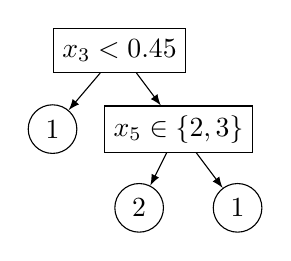
\begin{tikzpicture}
\node (labelleft) [draw,shape=circle,minimum size=16pt] at (2,0) {$2$};
\node (labelright) [draw,shape=circle,minimum size=16pt] at (3.25,0) {$1$};

\node (rootleft) [draw,shape=rectangle,minimum size=16pt] at (2.5,1) {$x_5 \in \{2,3\}$};
\node (rootlabel) [draw,shape=circle,minimum size=16pt] at (0.9,1) {$1$};
\node (root) [draw,shape=rectangle,minimum size=16pt] at (1.75,2) {$x_3 < 0.45$};

\draw[-latex] (root) -- (rootleft);
\draw[-latex] (root) -- (rootlabel);
\draw[-latex] (rootleft) -- (labelleft);
\draw[-latex] (rootleft) -- (labelright);

\end{tikzpicture}
\end{center}
\begin{center}
(a)
\end{center}
\end{minipage}
\hfill
\begin{minipage}{0.65\linewidth}
\begin{center}
\begin{tabular}{c|c|c|c|c|c|}
& Col 1 & Col 2 & Col 3 & Col 4 & Col 5\\
\hline
Row 1 & 1 & 2 & 3 & 6 & 7 \\
\hline
Row 2 & 1 & 0 & 1 & 0 & 0 \\
\hline
Row 3 & 3 & 5 & 0 & 0 & 0 \\
\hline
Row 4 & 1 & 1 & 2 & 2 & 1 \\
\hline
Row 5 & 1 & 0 & 2 & 0 & 0 \\
\hline
Row 6 & 0.45 & 0 & 2 & 0 & 0 \\
\hline
Row 7 &  &  & 3 &  & \\
\hline
\end{tabular}
\end{center}
\begin{center}
(b)
\end{center}
\end{minipage}
\caption{(a) An example tree and its (b) matrix representation. $x$ denotes an example and $x_j$ is the value of the $j$th continuous-valued (resp. categorical) feature in $X_\text{cont}$ (resp. $X_\text{cat}$). In this example all leaf nodes are pure and no training example is misclassified.}
\label{dtree}
\end{figure}


\smallskip
\noindent{\bf Returns}
\smallskip


The matrix corresponding to the learned model as well as the training accuracy (if requested) is written to a file in the format specified. See
details where the structure of the model matrix is described.
Recall that in our implementation $X$ is split into $X_\text{cont}$ and $X_\text{cat}$. If requested, the mappings of the continuous-valued feature-ids in $X_\text{cont}$ (stored at {\tt S\_map}) and the categorical feature-ids in $X_\text{cat}$ (stored at {\tt C\_map}) to the global feature-ids in $X$ will be provided. 
Depending on what arguments are provided during
invocation, the {\tt decision-tree-predict.dml} script may compute one or more of predictions, accuracy and confusion matrix in the requested output format. 

\smallskip
\noindent{\bf Examples}
\smallskip

{\hangindent=\parindent\noindent\tt
	\hml -f decision-tree.dml -nvargs X=/user/biadmin/X.mtx Y=/user/biadmin/Y.mtx
	R=/user/biadmin/R.csv M=/user/biadmin/model.csv
	bins=20 depth=25 num\_leaf=10 num\_samples=3000 impurity=Gini fmt=csv
	
}\smallskip


\noindent To compute predictions:

{\hangindent=\parindent\noindent\tt
	\hml -f decision-tree-predict.dml -nvargs X=/user/biadmin/X.mtx Y=/user/biadmin/Y.mtx R=/user/biadmin/R.csv
	M=/user/biadmin/model.csv  P=/user/biadmin/predictions.csv
	A=/user/biadmin/accuracy.csv CM=/user/biadmin/confusion.csv fmt=csv
	
}\smallskip


%\noindent{\bf References}
%
%\begin{itemize}
%\item B. Panda, J. Herbach, S. Basu, and R. Bayardo. \newblock{PLANET: massively parallel learning of tree ensembles with MapReduce}. In Proceedings of the VLDB Endowment, 2009.
%\item L. Breiman, J. Friedman, R. Olshen, and C. Stone. \newblock{Classification and Regression Trees}. Wadsworth and Brooks, 1984.
%\end{itemize}
